\documentclass[11pt]{article}
\usepackage[margin=2.5cm]{geometry}
\usepackage[utf8]{inputenc}
\usepackage[T1]{fontenc}
\usepackage{lmodern}
\usepackage{booktabs}
\usepackage{graphicx}

\title{Comparaison pr\'edictions vs valeurs r\'eelles \\ \large DeepEdgeBenchmark --- validation business}
\author{}
\date{Run du 7 juillet 2026 (holdout 7 jours)}

\begin{document}
\maketitle

\section{Objectif}

Ce rapport compl\`ete la validation business initiale~: au lieu de pr\'edire
depuis \guillemotleft{}aujourd'hui\guillemotright{} (o\`u le vrai futur n'est pas encore connu), les 7
derniers jours calendaires r\'eellement t\'el\'echarg\'es ont \'et\'e mis de
c\^ot\'e avant l'entra\^inement des mod\`eles (m\^eme logique que le
param\`etre T de \texttt{benchmarks/config.py}). Comme ces jours sont d\'ej\`a
connus dans les m\^emes donn\'ees, la vraie valeur (\texttt{actual}) est
disponible imm\'ediatement~: les pr\'edictions peuvent \^etre compar\'ees au
r\'eel sans attendre.

\section{P\'erim\`etre}

\begin{itemize}
  \item \textbf{Cutoff} : 2026-06-29 (holdout de 7 jours calendaires avant le
        dernier jour t\'el\'echarg\'e).
  \item \textbf{Actifs (5)} : BTC-USD, ETH-USD, SPY, ZN=F, TLT.
  \item \textbf{Horizons} : D+1 (r\'esolu pour les 5 actifs) et D+7 (r\'esolu
        seulement pour BTC-USD/ETH-USD --- voir \S\ref{sec:limite}).
  \item \textbf{Mod\`eles (5)} : ARIMA-GARCH, SARIMA, Prophet, LSTM, Naive.
\end{itemize}

\section{Erreur par mod\`ele (MAPE)}

\begin{table}[h]
\centering
\begin{tabular}{lrr}
\toprule
Mod\`ele & MAPE D+1 (5 actifs) & MAPE D+7 (BTC/ETH) \\
\midrule
Naive       & 1,16\,\% & 2,89\,\% \\
ARIMA-GARCH & 1,48\,\% & 7,21\,\% \\
SARIMA      & 1,53\,\% & 7,14\,\% \\
LSTM        & 1,56\,\% & 5,35\,\% \\
Prophet     & 20,03\,\% & 36,21\,\% \\
\bottomrule
\end{tabular}
\caption{Erreur absolue moyenne en \% (MAPE), tri\'ee par pr\'ecision \`a D+1.}
\end{table}

\`A D+1, les 4 mod\`eles statistiques/ML restent proches (1,2 \`a 1,6\,\%) ---
Naive fait m\^eme jeu \'egal, ce qui est attendu sur un horizon aussi court.
Prophet d\'ecroche massivement (20\,\% \`a D+1, 36\,\% \`a D+7), enti\`erement
port\'e par BTC-USD et ETH-USD (voir \S\ref{sec:prophet}).

\section{Graphique --- \'ecart pr\'ediction/r\'eel \`a D+1}

Le graphique ci-dessous montre, pour chaque actif et chaque mod\`ele, l'\'ecart
relatif entre la pr\'ediction \`a D+1 et la valeur r\'eellement observ\'ee.

\begin{figure}[h]
\centering
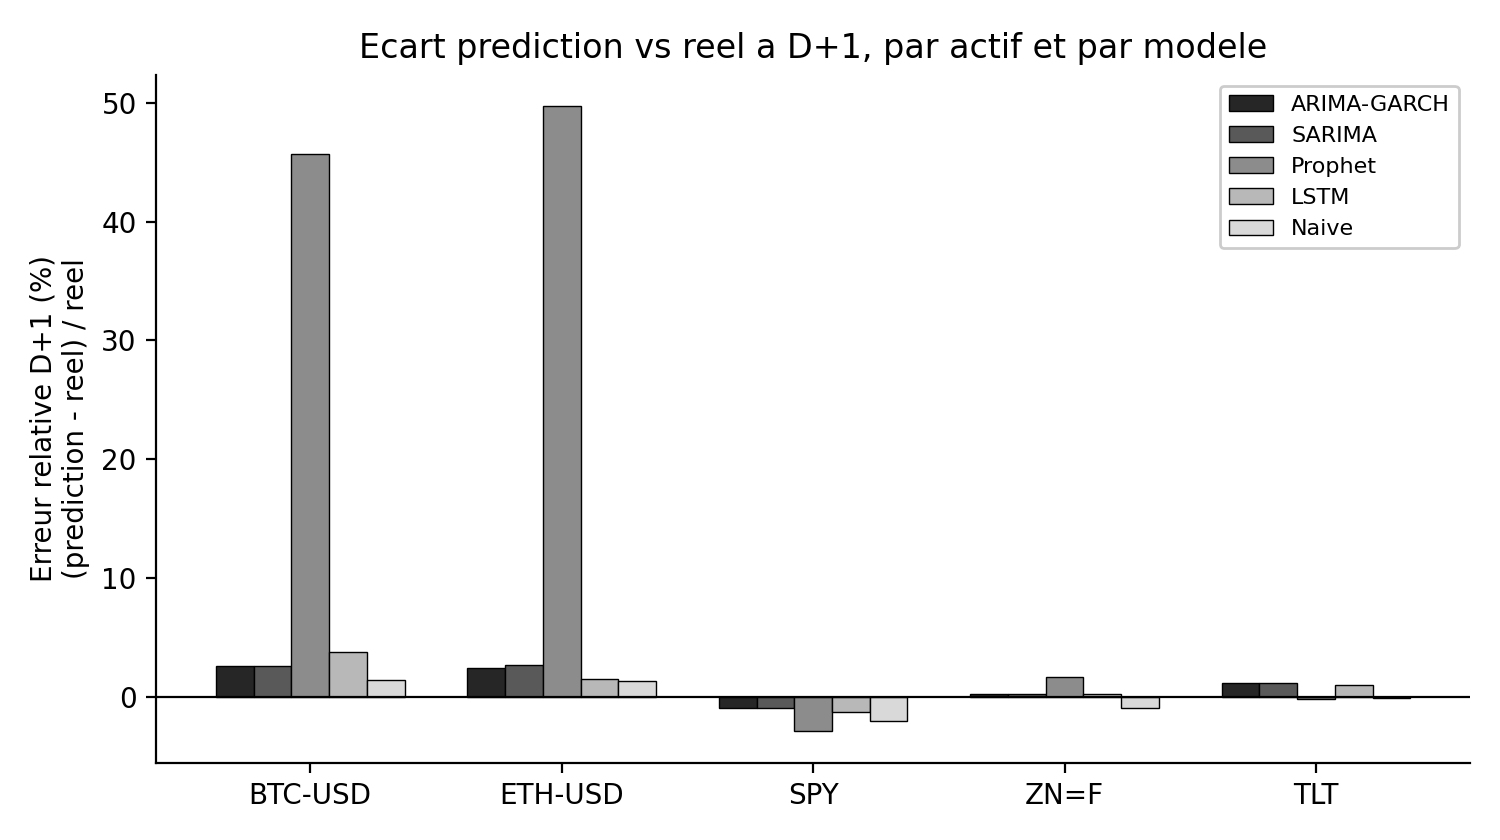
\includegraphics[width=0.95\textwidth]{chart_d1.png}
\caption{Erreur relative (pr\'ediction $-$ r\'eel) / r\'eel, par actif et par
mod\`ele, \`a D+1. Barres proches de 0 = pr\'ediction proche du r\'eel.}
\end{figure}

\section{Prophet sur BTC-USD/ETH-USD}
\label{sec:prophet}

\begin{table}[h]
\centering
\small
\begin{tabular}{llrrr}
\toprule
Actif & Horizon & Pr\'ediction & R\'eel & Erreur \\
\midrule
BTC-USD & D+1 & 85\,320 & 58\,559 & +45,7\,\% \\
BTC-USD & D+7 & 86\,531 & 63\,088 & +37,2\,\% \\
ETH-USD & D+1 & 2\,350  & 1\,570  & +49,7\,\% \\
ETH-USD & D+7 & 2\,406  & 1\,779  & +35,3\,\% \\
\bottomrule
\end{tabular}
\caption{Prophet surestime BTC-USD et ETH-USD de 35 \`a 50\,\% sur ce run.}
\end{table}

M\^eme diagnostic que dans le rapport pr\'ec\'edent~: Prophet fitte sur le prix
brut (pas le log-prix), avec une tendance lin\'eaire extrapol\'ee de mani\`ere
agressive sur des s\'eries \`a forte croissance non stationnaire comme
BTC/ETH. Sur les 3 autres actifs, Prophet reste dans le m\^eme ordre de
grandeur d'erreur que les autres mod\`eles (0,2 \`a 2,9\,\%).

\section{Limite de ce run --- D+7 non r\'esolu sur SPY/ZN=F/TLT}
\label{sec:limite}

Le holdout de 7 jours \emph{calendaires} cache 7 jours de trading pour les
cryptos (qui cotent tous les jours) mais seulement 4 jours de trading pour les
actifs qui ne cotent pas le week-end (SPY, ZN=F, TLT) --- il en faut 5 pour
r\'esoudre D+7. Cons\'equence~: sur ce run, D+7 reste \texttt{actual=NULL} pour
ces 3 actifs (15 test cases sur 50). Pour les couvrir syst\'ematiquement, il
faudrait un holdout d'au moins 9--10 jours calendaires (marge pour un jour
f\'eri\'e \'eventuel).

\section{Synth\`ese}

50 test cases g\'en\'er\'es, 0 \'echec technique. 35 r\'esolus (comparables au
r\'eel d\`es maintenant), 15 encore en attente (D+7 sur SPY/ZN=F/TLT). Hors
Prophet sur crypto, toutes les pr\'edictions restent dans un \'ecart de
quelques points de pourcentage du r\'eel \`a D+1 comme \`a D+7.

\end{document}
